\documentclass{beamer}
\usepackage{tikz,amsmath,hyperref,graphicx,stackrel,animate}
\usetikzlibrary{positioning,shadows,arrows,shapes,calc}
\newcommand{\argmax}{\operatornamewithlimits{argmax}}
\newcommand{\argmin}{\operatornamewithlimits{argmin}}
\mode<presentation>{\usetheme{Frankfurt}}
\AtBeginSection[]
{
  \begin{frame}<beamer>
    \frametitle{Outline}
    \tableofcontents[currentsection,currentsubsection]
  \end{frame}
}
\title{Lecture 3: Convolution}
\author{Mark Hasegawa-Johnson\\These slides are in the public domain.}
\date{ECE 401: Signal and Image Analysis}  
\begin{document}

% Title
\begin{frame}
  \maketitle
\end{frame}

% Title
\begin{frame}
  \tableofcontents
\end{frame}

%%%%%%%%%%%%%%%%%%%%%%%%%%%%%%%%%%%%%%%%%%%%
\section[Convolution]{Convolution}
\setcounter{subsection}{1}

\begin{frame}
  \frametitle{Convolution}
  \begin{itemize}
  \item A {\bf convolution} is exactly the same thing as a {\bf weighted local average}.
    We give it a special name, because we will use it very often.  It's defined as:
    \[
    y[n] = \sum_m g[m] f[n-m] = \sum_m g[n-m] f[m]
    \]
  \item 
    We use the symbol $\ast$ to mean ``convolution:''
    \[
    y[n]=g[n]\ast f[n] = \sum_m g[m] f[n-m] = \sum_m g[n-m] f[m]
    \]
  \end{itemize}
\end{frame}

\begin{frame}
  \frametitle{Convolution}
  \centerline{\fbox{$y[n] = g[n]\ast f[n] = \sum_m g[m] f[n-m] = \sum_m g[n-m] f[m]$}}

  \vspace*{2mm}
  
  Here is the pseudocode for convolution:
  \begin{enumerate}
  \item For every output $n$:
    \begin{enumerate}
    \item Reverse $g[m]$ in time, to create $g[-m]$.
    \item Shift it to the right by $n$ samples, to create $g[n-m]$.
    \item For every $m$:
      \begin{enumerate}
      \item Multiply $f[m]g[n-m]$.
      \end{enumerate}
    \item Add them up to create $y[n] = \sum_m g[n-m] f[m]$ for this particular $n$.
    \end{enumerate}
    \item Concatenate those samples together, in sequence, to make the signal $y$.
  \end{enumerate}
\end{frame}

%%%%%%%%%%%%%%%%%%%%%%%%%%%%%%%%%%%%%%%%%%%%
\section[Convolution]{Impulse Response}
\setcounter{subsection}{1}

\begin{frame}
  \frametitle{LSI Systems and Convolution}

  We care about linearity and shift-invariance because of the
  following remarkable result:
  \begin{block}{LSI Systems and Convolution}
    Let ${\mathcal H}$ be any system,
    \[
    x[n]\stackrel{H}{\longrightarrow} y[n]
    \]
    If ${\mathcal H}$ is linear and shift-invariant, then whatever
    processes it performs can be equivalently replaced by a
    convolution:
    \[
    y[n] = \sum_{m=-\infty}^\infty h[m] x[n-m]
    \]
  \end{block}
\end{frame}

\begin{frame}
  \frametitle{Impulse Response}

  \[
  y[n] = \sum_{m=-\infty}^\infty h[m] x[n-m]
  \]
  The weights $h[m]$ are called the ``impulse response'' of the
  system.  We can measure them, in the real world, by putting the
  following signal into the system:
  \[
  \delta[n] = \begin{cases} 1 & n=0\\ 0 & \mbox{otherwise}
  \end{cases}
  \]
  and measuring the response:
  \[
  \delta[n] \stackrel{H}{\longrightarrow} h[n]
  \]
\end{frame}



\begin{frame}
  \frametitle{Convolution: Proof}
  \begin{enumerate}
  \item $h[n]$ is the impulse response.
    \[
    \delta[n] \stackrel{H}{\longrightarrow} h[n]
    \]
  \item The system is {\bf shift-invariant}, therefore
    \[
    \delta[n-m] \stackrel{H}{\longrightarrow} h[n-m]
    \]
  \item The system is {\bf linear}, therefore {\bf scaling the input
    by a constant} results in {\bf scaling the output by the same
    constant}:
    \[
    x[m]\delta[n-m] \stackrel{H}{\longrightarrow} x[m]h[n-m]
    \]
  \item The system is {\bf linear}, therefore {\bf adding input
    signals} results in {\bf adding the output signals}:
    \[
    \sum_{m=-\infty}^\infty x[m]\delta[n-m]
    \stackrel{H}{\longrightarrow} \sum_{m=-\infty}^\infty x[m]h[n-m]
    \]
  \end{enumerate}
\end{frame}

\begin{frame}
  \frametitle{Convolution: Proof (in Words)}

  \begin{itemize}
  \item The input signal, $x[n]$, is just a bunch of samples.
  \item Each one of those samples is a scaled impulse, so each one of
    them produces a scaled impulse response at the output.
  \item Convolution = add together those scaled impulse responses.
  \end{itemize}
\end{frame}


\begin{frame}
  \frametitle{Convolution: Proof (in Pictures)}

  \centerline{\includegraphics[width=\textwidth]{exp/convolutionproof.png}}
\end{frame}

%%%%%%%%%%%%%%%%%%%%%%%%%%%%%%%%%%%%%%%%%%%%
\section[Graphical]{Graphical Convolution}
\setcounter{subsection}{1}

\begin{frame}
  \frametitle{Convolution: how should you implement it?}

  \begin{itemize}
    \item 
      When writing code: use the numpy function, {\tt np.convolve}.
      In general, if numpy has a function that solves your problem,
      you are {\em always} permitted to use it.
    \item
      When solving problems with pencil and paper: use {\em graphical
        convolution}.
  \end{itemize}
\end{frame}

\begin{frame}
  \frametitle{Graphical Convolution}

  \begin{enumerate}
  \item Choose one of the two functions whose breakpoints are easier to shift
    (i.e., it breaks at easy values like $n=0$), and call that $f[n]$.  Call the other
    function $g[n]$.
  \item Plot $g[m]$ as a function of $m$.
  \item Underneath, plot $f[n-m]$
    as a function of $m$ for some particular $n$.
  \item Under that, plot $g[m]f[n-m]$ for the same particular $n$.
  \item Use your plot as a guide to help you write the equation
    $\sum_m g[m]f[n-m]$ in a solvable form.  Solve it to find $y[n]$.
  \item If this gives you enough information to find $y[n]$ for every
    other $n$, then do so.  If there's some other $n$ that's not yet
    obvious to you, then repeat above process for the other $n$.
  \end{enumerate}
\end{frame}

\begin{frame}
  \frametitle{Graphical Convolution: A Video from Wikipedia}
  \animategraphics[loop,controls,width=\linewidth]{20}{exp/convolution-}{0}{279}
  \begin{tiny}
    by Brian Amberg, CC-SA 3.0,
    \url{https://commons.wikimedia.org/wiki/File:Convolution_of_spiky_function_with_box2.gif}
  \end{tiny}
\end{frame}

\begin{frame}
  \frametitle{Quiz}

  Do the quiz!  Go to the course webpage, and try the quiz.
\end{frame}


%%%%%%%%%%%%%%%%%%%%%%%%%%%%%%%%%%%%%%%%%%%%
\section[Differencing]{Differencing}
\setcounter{subsection}{1}

\begin{frame}
  \frametitle{Differencing is convolution, too}

  Suppose we want to compute the local difference:
  \[
  y[n] = f[n] - f[n-1]
  \]
  We can do that using a convolution!
  \[
  y[n] = \sum_m f[n-m]h[m]
  \]
  where
  \[
  h[m] = \begin{cases}
    1 & m=0\\
    -1 & m=1\\
    0 & \mbox{otherwise}
  \end{cases}
  \]
\end{frame}

\begin{frame}
  \frametitle{Differencing as convolution} 
  \centerline{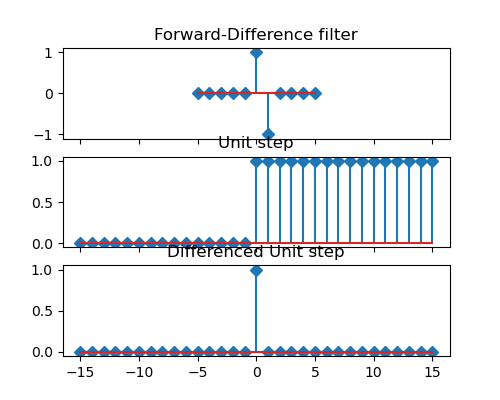
\includegraphics[height=2.5in]{mp3fig5.png}}
\end{frame}
  
%%%%%%%%%%%%%%%%%%%%%%%%%%%%%%%%%%%%%%%%%%%%
\section[Weighted]{Weighted Differencing}
\setcounter{subsection}{1}

\begin{frame}
  \frametitle{Weighted differencing as convolution}
  \begin{itemize}
    \item 
      The formula $y[n]=f[n]-f[n-1]$ is kind of noisy.  Any noise in
      $f[n]$ or $f[n-1]$ means noise in the output.
    \item
      We can make it less noisy  by
      \begin{enumerate}
      \item First, compute a weighted average:
        \[
        y[n] = \sum_m f[m]g[n-m]
        \]
      \item Then, compute a local difference:
        \[
        z[n] = y[n] - y[n-1] = \sum_m f[m]\left(g[n-m]-g[n-1-m]\right)
        \]
      \end{enumerate}
      This is exactly the same thing as convolving with
      \[
      h[n] = g[n]-g[n-1]
      \]
  \end{itemize}
\end{frame}

\begin{frame}
  \frametitle{A difference-of-Gaussians filter}

  The top row is a ``difference of Gaussians'' filter,
  $h[n]=g[n]-g[n-1]$, where $g[n]$ is a Gaussian.  The middle row is
  $f[n]$, the last row is the output $z[n]$.
  \centerline{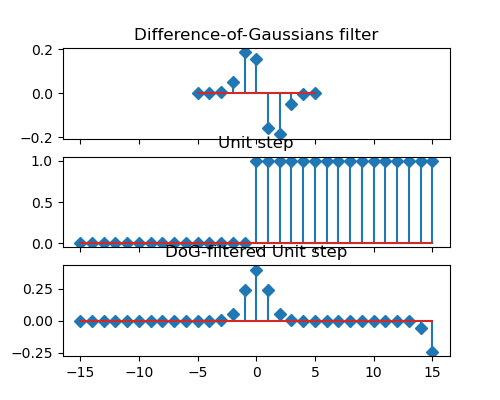
\includegraphics[height=2.5in]{mp3fig7.png}}
\end{frame}

\begin{frame}
  \frametitle{Difference-of-Gaussians filtering in both rows and columns}
      
  \centerline{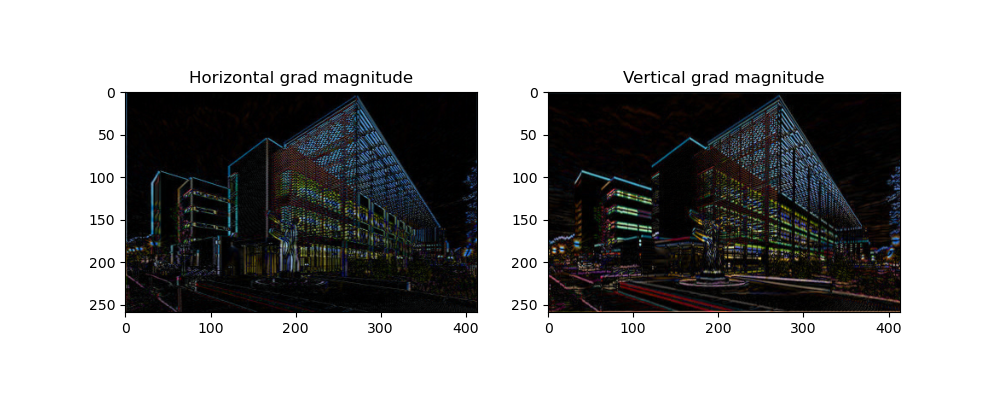
\includegraphics[height=2.5in]{mp3fig8.png}}
\end{frame}

%%%%%%%%%%%%%%%%%%%%%%%%%%%%%%%%%%%%%%%%%%%%
\section[Edges]{Edge Detection}
\setcounter{subsection}{1}

\begin{frame}
  \frametitle{Image gradient}
  \begin{itemize}
  \item Suppose we have an image $f[i,j,k]$.  The 2D image gradient is
    defined to be
    \[
    \vec{G}[i,j,k] = \left(\frac{df}{di}\right)\hat{i} + \left(\frac{df}{dj}\right)\hat{j}
    \]
    where $\hat{i}$ is a unit vector in the $i$ direction, $\hat{j}$
    is a unit vector in the $j$ direction.
  \item We can approximate these using the difference-of-Gaussians filter, $h_{dog}[n]$:
    \begin{align*}
      \frac{df}{di} &\approx G_i = h_{dog}[i]\ast f[i,j,k]\\
      \frac{df}{dj} &\approx G_j = h_{dog}[j]\ast f[i,j,k]\\
    \end{align*}
  \end{itemize}
\end{frame}
\begin{frame}
  \frametitle{The gradient is a vector}
  The image gradient, at any given pixel, is a vector.  It  points in the direction of
  increasing intensity (this image shows ``dark'' = greater intensity).
  \centerline{
\includegraphics[height=2in]{exp/gradient.png}}
  \begin{tiny}
    By CWeiske, CC-SA 2.5,
    \url{https://commons.wikimedia.org/wiki/File:Gradient2.svg}
  \end{tiny}
\end{frame}
      
\begin{frame}
  \frametitle{Magnitude of the image gradient}
  \begin{itemize}
  \item
    The image gradient, at any given pixel, is a vector.
  \item
    It points in the direction in which intensity is increasing.
  \item
    The magnitude of the vector tells you how fast intensity is
    changing.
    \[
    \Vert \vec{G}\Vert =\sqrt{G_i^2 + G_j^2}
    \]
  \end{itemize}
\end{frame}
    
\begin{frame}
  \frametitle{Magnitude of the gradient = edge detector}
      
  \centerline{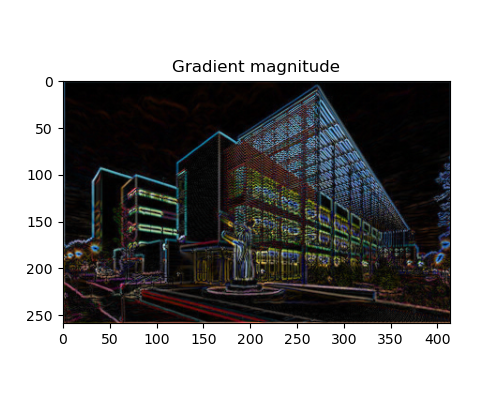
\includegraphics[height=3.5in]{mp3fig9.png}}
\end{frame}

%%%%%%%%%%%%%%%%%%%%%%%%%%%%%%%%%%%%%%%%%%%%
\section[Summary]{Summary}
\setcounter{subsection}{1}
\begin{frame}
  \frametitle{Summary}

  If a system is {\bf linear and shift-invariant} (LSI), then it can
  be implemented using convolution:
    \[
    y[n] = h[n]\ast x[n] = \sum_m h[m] x[n-m] = \sum_m h[n-m] x[m]
    \]
    where $h[n]$ is the impulse response:
    \[
    \delta[n] \stackrel{\mathcal H}{\longrightarrow}  h[n]
    \]
\end{frame}

\end{document}
